\subsection*{Case 4} % Aktia 
\label{case: 4}
% deployment setup diagram
% \begin{figure*}[t]
% \centering
% 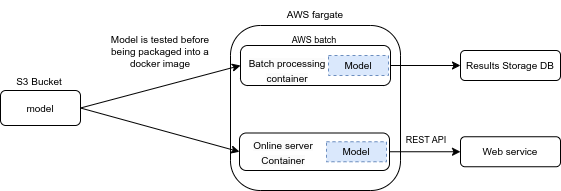
\includegraphics[width=0.8\textwidth]{images/case4_deployment_process_v2.png}
% \caption{Case 4 deployment setup}
% \label{fig: case4_deployment_process}
% \end{figure*}

% Case description: Inscripta 
% deployment setup diagram
\begin{figure*}[t]
\centering
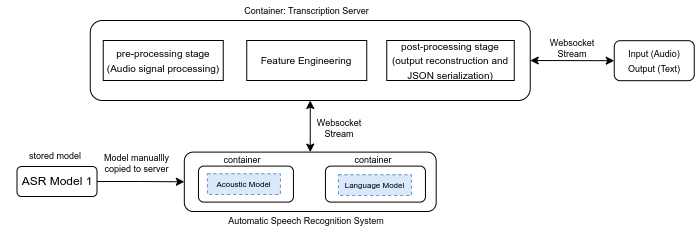
\includegraphics[width=0.8\textwidth]{images/case3_deployment_process_v2.png}
\caption{Case 3 Inference Architecture}
\label{fig: case3_deployment_process}
\end{figure*}

The ML system generates risk classification profiles of clients in financial services setting. This system is part of a broader microservices supporting analytics and predictive risk management services. Financial services are typically regulated, imposing explainability requirements on algorithms and models used to support business process decision-making. The models are trained from data obtained from internal systems. The inference results are stored in an internal datalake accessible to other software components in the broader ecosystem. 

\textit{Pre-integration}: The entire process is centred on a CI/CD pipeline (Atlassian Bamboo) that first involves building the model code into a docker container for the training workflow. The building process is managed with a custom shell or Python scripts. The resulting model artefact moves to a quality assurance stage, which is tested before being serialized and stored in a versioned S3 bucket. Models are updated routinely based on a schedule (weekly, monthly) or based on business demands; the routine updates are based on re-training workflows configured with Airflow.

\textit{Quality assurance}: Other sanity and basic tests are carried out before the model is deployed. This may involve checking metrics (MAE, RMSE) or resulting data distributions.
The versioned storage allows tracking changes in the model artefact to increase the traceability of models due to regulatory demands. 

\textit{Server environment}: A model is deployed in two configurations: i) batch inference processing and ii) as an online prediction service. The batch deployment uses AWS batch and AWS Fargate services to run the batch inference jobs. AWS batch provides the scheduling functionality, while the AWS Fargate provides a serverless container computing environment. The online prediction model is a containerized Python-based server. 

\textit{Inference}: Batch inference jobs are executed regularly on a weekly or monthly basis to generate predictions using pre-processed input data stored in a data lake, and the inference results are stored back into the data lake. The process involves direct access (through function calls) to a serialized model object without using web-based endpoints.
Online inference, on the other hand, is performed through a REST API endpoint that provides real-time predictions to users. This is achieved by sending requests to the API endpoint and receiving immediate responses. This inference architecture is shown in Figure~\ref{fig: case4_deployment_process}.

\textit{Monitoring}: The monitoring setup includes an API gateway to monitor and secure the real-time endpoint and a dashboard that aggregates model metrics such as drift. In addition, other monitoring aspects are handled using Splunk, including monitoring batch run’s success/failure and responsiveness of live endpoint runs, among others.
